\documentclass[conference]{IEEEtran}
%DIF LATEXDIFF DIFFERENCE FILE
%DIF DEL paper/v1-initial/main.tex   Wed Nov 25 20:29:36 2026
%DIF ADD paper/v2-revised/main.tex   Wed Nov 25 20:29:36 2026
\usepackage[T1]{fontenc}
%DIF 3c3
%DIF < \usepackage{cite,amsmath,amssymb,graphicx,booktabs,url,balance}
%DIF -------
\usepackage{array,cite,amsmath,amssymb,graphicx,booktabs,url,balance} %DIF > 
%DIF -------
\usepackage{tikz}
\usetikzlibrary{arrows.meta,positioning,shapes.geometric,fit}
\newcommand{\sys}{SmartIntake}
\newcommand{\pending}{\textit{planned; not measured}}
\hyphenation{Post-gre-SQL Fast-API Smart-Intake}
%DIF 9a9
\newcolumntype{P}[1]{>{\raggedright\arraybackslash}p{#1}} %DIF > 
%DIF -------
\newenvironment{DIFnomarkup}{}{}
%DIF PREAMBLE EXTENSION ADDED BY LATEXDIFF
%DIF CFONT PREAMBLE %DIF PREAMBLE
\RequirePackage{color}\definecolor{RED}{rgb}{1,0,0}\definecolor{BLUE}{rgb}{0,0,1} %DIF PREAMBLE
\DeclareOldFontCommand{\sf}{\normalfont\sffamily}{\mathsf} %DIF PREAMBLE
\providecommand{\DIFadd}[1]{{\protect\color{blue} \sf #1}} %DIF PREAMBLE
\providecommand{\DIFdel}[1]{{\protect\color{red} \ifmmode #1\else\scriptsize #1\fi}} %DIF PREAMBLE
%DIF SAFE PREAMBLE %DIF PREAMBLE
\providecommand{\DIFaddbegin}{} %DIF PREAMBLE
\providecommand{\DIFaddend}{} %DIF PREAMBLE
\providecommand{\DIFdelbegin}{} %DIF PREAMBLE
\providecommand{\DIFdelend}{} %DIF PREAMBLE
\providecommand{\DIFmodbegin}{} %DIF PREAMBLE
\providecommand{\DIFmodend}{} %DIF PREAMBLE
%DIF FLOATSAFE PREAMBLE %DIF PREAMBLE
\providecommand{\DIFaddFL}[1]{\DIFadd{#1}} %DIF PREAMBLE
\providecommand{\DIFdelFL}[1]{\DIFdel{#1}} %DIF PREAMBLE
\providecommand{\DIFaddbeginFL}{} %DIF PREAMBLE
\providecommand{\DIFaddendFL}{} %DIF PREAMBLE
\providecommand{\DIFdelbeginFL}{} %DIF PREAMBLE
\providecommand{\DIFdelendFL}{} %DIF PREAMBLE
%DIF END PREAMBLE EXTENSION ADDED BY LATEXDIFF

\hyphenation{Tool-for-mer}
\begin{document}
\title{SmartIntake: An IoT and Tool-Grounded AI Agent-Based System for Hydration and Dietary Tracking}
\author{\IEEEauthorblockN{[Authors pending confirmation]}
\IEEEauthorblockA{[Affiliations and contact pending confirmation]}}
\maketitle
\begin{abstract}
Manual hydration and dietary recording imposes repeated interaction costs, while weight sensing alone cannot establish whether a person consumed a measured mass loss. This paper proposes SmartIntake, a fixed-workplace system combining a Raspberry Pi 4 and two independent Load Cell/HX711 scales with FastAPI, Supabase PostgreSQL, Discord, and an n8n tool-grounded language agent. A finite-state sensing process generates candidate drinking events; correction and confirmation preserve the distinction between observations and recorded intake. Food entry uses tared net mass or explicitly labeled reference portions. Versioned shared-device sessions separate physical event attribution from the authenticated identity of a person asking a question. Read-only agent tools delegate arithmetic and authorization to the backend and return record-level provenance and missing-data indicators. We define five prospective evaluations covering weight accuracy, event detection, switching consistency, recording burden, and agent reliability. The contribution is an integrated research design and evaluation framework, not a validated health intervention. Formal experimental results and implementation verification remain pending.
\end{abstract}

\begin{IEEEkeywords}Internet of Things, hydration tracking, dietary recording, load cell, tool-grounded agent, provenance\end{IEEEkeywords}
\section{Introduction}\label{sec:intro}
Hydration and food diaries require people to repeatedly notice an event, identify a quantity, and enter a record. Dietary self-monitoring has been studied extensively, but heterogeneous methods and adherence measures complicate interpretation~\cite{burke2011}. Lower interaction effort is therefore a design objective rather than evidence that a particular interface improves health. A laboratory or office offers an opportunity to instrument recurring routines without requiring a dedicated bottle to travel with every user.

Two problems remain when a scale replaces manual quantity entry. First, a decrease in container mass may reflect drinking, discarding water, spilling, or replacing the container. Commercial bottle evaluation has explicitly identified this distinction and the dependence on returning a bottle to a surface~\cite{cohen2022}. Second, a shared scale measures an object, not an authenticated person. Even accurate mass estimates can produce misleading personal histories if a user switches during an event. Conversational access adds another failure path: a fluent summary can conceal missing records, inconsistent units, or unauthorized queries.

\sys{} addresses these concerns as a proposed fixed-workplace research system. One scale acts as a drinking-cup station and the other supports food weighing. A Raspberry Pi 4 runs sensor acquisition; FastAPI mediates ingestion, authorization, event processing, and deterministic calculations; Supabase provides PostgreSQL storage. Discord supplies selection and correction interactions. An n8n agent chooses read-only analytics tools and explains returned evidence. We do not propose a new language model or a new load-cell transducer.

The study asks: \textbf{RQ1}, can temporal sensing and event confirmation improve hydration recording in the presence of ambiguous mass changes? \textbf{RQ2}, can versioned shared-device attribution and semi-automatic entry support reliable records with less interaction than manual entry? \textbf{RQ3}, can tool-grounded summaries preserve numeric correctness, authorization, and provenance?

The paper contributes (1) a sensing-to-record architecture that preserves uncertainty and correction history, (2) a method combining mass-based candidate events, food portion semantics, and session-based attribution, and (3) a prospective E1--E5 evaluation linking sensing and conversational failures to observable metrics. Tool use is motivated by ReAct and Toolformer~\cite{yao2023react,schick2023}; it does not by itself establish truthful or authorized behavior. All components below describe a proposed design. No formal E1--E5 measurements or independently verified running deployment are reported.

\DIFaddbegin \begin{table}[t]
\caption{\DIFaddFL{Research questions and primary prospective outcomes. All outcomes remain unmeasured.}}\label{tab:questions}
\centering\footnotesize\setlength{\tabcolsep}{4pt}
\begin{tabular}{@{}P{.10\columnwidth}P{.56\columnwidth}P{.25\columnwidth}@{}}\toprule
\DIFaddFL{RQ }& \DIFaddFL{Primary outcome / obligation }& \DIFaddFL{Evaluation}\\\midrule
\DIFaddFL{1 }& \DIFaddFL{Final-record F1 alongside candidate F1 and prompt burden }& \DIFaddFL{E1 calibration; E2 detection}\\
\DIFaddFL{2 }& \DIFaddFL{Wrong-owner rate with resolved coverage; paired task time with completion }& \DIFaddFL{E3 switching; E4 effort}\\
\DIFaddFL{3 }& \DIFaddFL{Strict all-component run success and three-repeat case reliability }& \DIFaddFL{E5 agent tests}\\\bottomrule
\end{tabular}
\end{table}
\DIFadd{Table~\ref{tab:questions} makes the integration contribution falsifiable. A method that improves apparent F1 by withholding unresolved events, or reduces reported time by omitting corrections, would not satisfy these obligations. The study does not establish a superior sensing algorithm or general-purpose agent.
}

\DIFaddend \section{Related Work}\label{sec:related}
\subsection{Hydration and Dietary Self-Monitoring}
Playful Bottle explored office hydration through a phone attached to a mug, vision/motion sensing, and social persuasion~\cite{chiu2009}. This establishes relevant workplace context, but its sensing and persuasive-interaction objectives differ from a shared stationary weighing service. Cohen \textit{et al.} compared commercial smart bottles against a reference scale and discussed missed records and ambiguous liquid loss~\cite{cohen2022}. Their study motivates separate checks of quantity accuracy and event interpretation; its results cannot be transferred to the proposed hardware.

Burke \textit{et al.} reviewed dietary, exercise, and weight self-monitoring and emphasized methodological limitations and adherence measurement~\cite{burke2011}. For \sys{}, a shorter entry procedure is a hypothesis to test with observed tasks. Food mass also requires an identified item and a documented nutrient basis: a scale cannot infer a mixed meal's composition. FoodData Central documents multiple data types and their provenance~\cite{usda}; records should retain the selected food identifier and data release rather than treat a generated food description as a nutrient source.

\subsection{Tool Use and Provenance}
ReAct interleaves language-model reasoning and actions, while Toolformer studies learning when and how to invoke APIs~\cite{yao2023react,schick2023}. We adopt the narrower engineering principle that external tools should supply facts and arithmetic. We do not claim to reproduce those training procedures. The $\tau$-bench study evaluates tool-agent-user interactions and repeated reliability under domain policies~\cite{yao2024tau}; it motivates testing more than a single successful conversation. W3C PROV-DM distinguishes entities, activities, derivation, and responsible agents~\cite{prov}. This informs our provenance chain without claiming formal PROV conformance.

\begin{table}[t]
\caption{Selected research perspectives and their relevance. The final column is our design interpretation, not a benchmark result.}\label{tab:related}
\centering\footnotesize\setlength{\tabcolsep}{4pt}
\DIFdelbeginFL %DIFDELCMD < \begin{tabular}{@{}p{.19\columnwidth}p{.31\columnwidth}p{.42\columnwidth}@{}}%%%
\DIFdelendFL \DIFaddbeginFL \begin{tabular}{@{}P{.19\columnwidth}P{.31\columnwidth}P{.42\columnwidth}@{}}\DIFaddendFL \toprule
Work & Studied focus & SmartIntake design implication\\\midrule
\DIFdelbeginFL \DIFdelFL{Playful }\DIFdelendFL Bottle~\cite{chiu2009} & Workplace sensing and persuasion & Examine routine recording in a fixed setting\\
Smart bottles~\cite{cohen2022} & Quantity and recording accuracy & Separate mass accuracy from ingestion labels\\
\DIFdelbeginFL \DIFdelFL{ReAct / Toolformer}\DIFdelendFL \DIFaddbeginFL \DIFaddFL{Tools}\DIFaddendFL ~\cite{yao2023react,schick2023} & Model interaction with tools & Keep arithmetic in backend tools\\
$\tau$-bench~\cite{yao2024tau} & Policy and repeated agent reliability & Test authorization and repeatability\\\bottomrule
\end{tabular}
\end{table}

The gap addressed here is the joint treatment of ambiguous stationary sensing, shared-device attribution, and evidence-preserving conversational retrieval within this selected literature. This is a scoped integration contribution; it is not a claim that no prior system combines these features.

\DIFaddbegin \DIFadd{The distinction is operational: the hydration comparison motivates an independent physical oracle (E1/E2), workplace interaction motivates a measured effort comparison (E4), and policy-oriented tool evaluation motivates subject isolation and repeated scoring (E5). Combining these concerns imposes session coordination and query-snapshot obligations that are specified below. This is our synthesis of the selected works, not evidence that those works lack every related mechanism.
}

\DIFaddend \section{System Architecture}\label{sec:architecture}
Figure~\ref{fig:architecture} shows the proposed data path and trust boundaries. Two separate Load Cell/HX711 assemblies connect to a Raspberry Pi 4: one for hydration and one for food. A Python worker calibrates readings, estimates stable mass, detects temporal transitions, and queues observations during outages. Calibration and device identifiers accompany events. Hardware capacity, mounting, sample rate, and measured stability must be documented when the prototype is built.

\begin{figure*}[t]
\centering
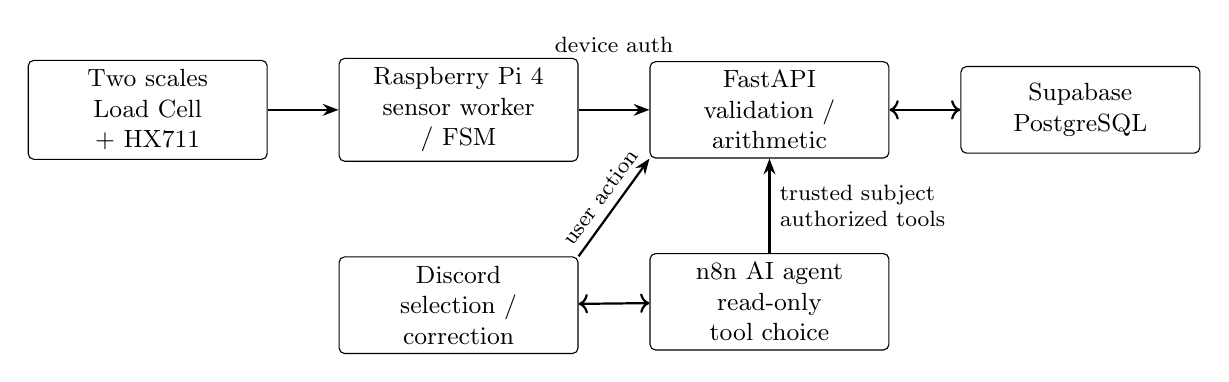
\begin{tikzpicture}[font=\small,box/.style={draw,rounded corners=2pt,align=center,minimum height=11mm,text width=28mm},arr/.style={-{Stealth[length=2mm]},thick}]
\node[box] (s) {Two scales\\Load Cell + HX711};
\node[box,right=9mm of s] (p) {Raspberry Pi 4\\sensor worker / FSM};
\node[box,right=9mm of p] (a) {FastAPI\\validation / arithmetic};
\node[box,right=9mm of a] (d) {Supabase\\PostgreSQL};
\node[box,below=12mm of p] (u) {Discord\\selection / correction};
\node[box,below=12mm of a] (n) {n8n AI agent\\read-only tool choice};
\draw[arr] (s)--(p);\draw[arr] (p)--node[above=6mm,font=\footnotesize]{device auth}(a);\draw[arr,<->] (a)--(d);
\draw[arr,<->] (u)--(n);\draw[arr] (n)--node[right,font=\footnotesize,align=left]{trusted subject\\authorized tools}(a);
\draw[arr] (u.north east)--node[above,sloped,font=\footnotesize]{user action}(a.south west);
\end{tikzpicture}
\caption{Proposed architecture. User actions and agent queries cross separate authorization paths; physical observations do not establish ingestion or identity by themselves.}\label{fig:architecture}
\end{figure*}


FastAPI accepts authenticated device events and user actions. Supabase PostgreSQL stores observations, candidate events, device-session versions, food definitions, confirmed or inferred records, and append-only corrections. A unique event identifier prevents duplicate ingestion on retries. Storage is a design choice; neither a deployed schema nor transactional behavior has been verified in this study.

The Discord interaction layer authenticates the person selecting an active session, choosing food, confirming an ambiguous event, or reversing an inferred record. Three users share the two scales in the intended pilot. The active physical session applies to both scales. The identity used for a conversational query remains the authenticated Discord requestor, independent of whoever currently owns the scales. Changing the active session must not redirect another person's analytics request.

The n8n workflow routes a question to an allowlisted tool service. Six read-only tool functions cover daily hydration, hydration history, food history, nutrition summaries, goal progress, and record sources. FastAPI derives the authorized subject from trusted service and user context; a language-model-generated user identifier has no authority. Calculations and date filtering occur behind that boundary. Tools return data, units, sources, warnings, and explicit statuses distinguishing success, no data, forbidden access, invalid requests, and upstream failures.

Raw scale data and personal food histories are sensitive. Devices should receive only ingestion privileges, and agent credentials should expose only the minimum read operations. Supabase service-role credentials must remain server-side. Neither a bot token nor a workflow export containing credentials belongs in the public manuscript package. The proposed architecture requires authenticated transport, request validation, and access isolation; these are requirements for future implementation tests, not security certification.

\section{Proposed Methodology}\label{sec:method}
\subsection{Calibration and Stable Observations}
Let $r_i$ be an HX711 reading and \DIFdelbegin \DIFdel{let }\DIFdelend $\hat m_i$ \DIFdelbegin \DIFdel{be }\DIFdelend calibrated mass in \DIFdelbegin \DIFdel{grams. A linear model fitted from reference masses is
}\DIFdelend \DIFaddbegin \DIFadd{g. Fit a linear per-scale model using reference loads,
}\DIFaddend \begin{equation}\hat m_i=a r_i+b.\label{eq:calibration}\end{equation}
\DIFdelbegin \DIFdel{The coefficients belong to a specific scale and mounting configuration. Repeated placements and zero-load checks are needed to characterize drift. }\DIFdelend A median over \DIFdelbegin \DIFdel{a sliding window suppresses isolated disturbances}\DIFdelend \DIFaddbegin \DIFadd{$W$ samples estimates stable mass}\DIFaddend . A window is \DIFdelbegin \DIFdel{stable only when its range is below a calibrated tolerance }\DIFdelend \DIFaddbegin \DIFadd{valid only if all samples are valid, within the documented operating range, and its range remains at most }\DIFaddend $\epsilon$ for \DIFdelbegin \DIFdel{a }\DIFdelend dwell time $T_s$\DIFdelbegin \DIFdel{; unstable windows cannot finalize a quantity. Parameters are to be selected using calibration trials and fixed before evaluation, not chosen to improve reported test scores}\DIFdelend . \DIFaddbegin \DIFadd{Saturation, stale samples and sensor errors invalidate it. A reference must be reacquired after restart, remounting or container reset. Calibration coefficients and uncertainty belong to one scale/mounting version.
}\DIFaddend 

\DIFdelbegin \subsection{\DIFdel{Hydration Candidate Events}}
%DIFAUXCMD
\addtocounter{subsection}{-1}%DIFAUXCMD
\DIFdel{A finite-state machine (FSM) records a stable pre-lift mass, observes absence }\DIFdelend \DIFaddbegin \DIFadd{The pre-test parameter manifest must freeze sampling rate $f_s$, window size $W$}\DIFaddend , \DIFdelbegin \DIFdel{waits for return, and requires a stable post-return mass (Fig. ~\ref{fig:fsm}). The event begins at the lift transition . A short interval of unstable contact must not generate repeated lift events. For an unchanged vessel }\DIFdelend \DIFaddbegin \DIFadd{$\epsilon$}\DIFaddend , \DIFdelbegin \begin{displaymath}\DIFdel{\Delta m=\bar m_{\rm before}-\bar m_{\rm after},\qquad
\hat V=\frac{\Delta m}{\rho},%DIFDELCMD < \label{eq:volume}%%%
}\end{displaymath}%DIFAUXCMD
\DIFdelend \DIFaddbegin \DIFadd{$T_s$, absence threshold $\theta_L$, minimum positive difference $\theta_D$, maximum absence duration $T_A$, allowed mass range $[0,M]$, and density approximation $\rho$. Presence requires stable mass above $\theta_L$; absence requires mass below it for $T_s$. Values depend on calibration and the chosen vessel, and are not supplied as validated constants. A setup pilot selects them before held-out evaluation; every change creates a new manifest version.
}

\subsection{\DIFadd{Hydration Lifecycle and Candidate Events}}
\DIFadd{Figure~\ref{fig:fsm} remains a high-level workflow; Table~\ref{tab:states} defines its lifecycle guards. The lift transition durably binds the pre-lift observations, calibration and session grant to a unique event. The sensor continues observing an in-flight event through a user switch. Invalid or unresolved comparisons cannot establish a new inferred-intake baseline without explicit reset and reacquisition.
}

\begin{DIFnomarkup}\begingroup\color{blue}\begin{table*}[t]\color{blue}
\caption{Proposed hydration lifecycle. Parameters are calibrated and frozen before evaluation; no threshold value is claimed as measured.}\label{tab:states}
\centering\footnotesize\setlength{\tabcolsep}{4pt}
\begin{tabular}{@{}P{.13\textwidth}P{.35\textwidth}P{.44\textwidth}@{}}\toprule
State & Guard / next state & Output and re-arming rule\\\midrule
INIT & Valid stable vessel and current grant $\to$ PRESENT & Acquire baseline; no intake output. Invalid input stays INIT.\\
PRESENT & Absence for $T_s$ $\to$ ABSENT & Start one durable event and bind pre-mass/session; contact noise leaves state unchanged.\\
ABSENT & Return before $T_A$ $\to$ RETURN; timeout $\to$ RESOLVE & Retain pre-mass and owner; do not create repeated lift events.\\
RETURN & Stable valid window $\to$ CLASSIFY; new loss $\to$ ABSENT & No quantity until stable; the original timeout bounds the entire event.\\
CLASSIFY & Valid vessel/range and $\Delta m$ $\to$ disposition; otherwise RESOLVE & Candidate, refill-like or no-change; save evidence and enter PRESENT with the validated post-mass.\\
RESOLVE & Explicit user resolution/reset plus stable reacquisition $\to$ INIT & No inferred intake from invalid comparison; vessel changes always require reset.\\\bottomrule
\end{tabular}
\end{table*}
\endgroup\end{DIFnomarkup}

\DIFadd{For a consistent vessel and two valid stable masses,
}\begin{equation}\DIFadd{\Delta m=\bar m_{\rm before}-\bar m_{\rm after},\qquad
\hat V=\frac{\Delta m}{\rho}.\label{eq:volume}}\end{equation}\DIFaddend 
\DIFdelbegin \DIFdel{where mass is in g, }\DIFdelend \DIFaddbegin \DIFadd{Here }\DIFaddend $\rho$ is \DIFdelbegin \DIFdel{the declared water-density approximation }\DIFdelend in g/mL \DIFdelbegin \DIFdel{, }\DIFdelend and $\hat V$ \DIFdelbegin \DIFdel{is a candidate volume }\DIFdelend in mL. \DIFdelbegin \DIFdel{Using }\DIFdelend \DIFaddbegin \DIFadd{The approximation }\DIFaddend $\rho\approx1$ is \DIFdelbegin \DIFdel{an engineering approximation for water , not a measured density for arbitrary beverages. The vessel-cancellation assumption fails after a container change.
}%DIFDELCMD < 

%DIFDELCMD < %%%
\DIFdel{A positive change above a calibrated detection threshold }\DIFdelend \DIFaddbegin \DIFadd{declared for water only. A positive $\Delta m>\theta_D$ within the plausible range }\DIFaddend produces a candidate\DIFdelbegin \DIFdel{. A negative change suggests refill; a near-zero change is ignored. A timeout, implausible change, or inconsistent vesselcontext is routed for confirmation rather than silently counted. A putative }\DIFdelend \DIFaddbegin \DIFadd{; $\Delta m<-\theta_D$ is refill-like, and $|\Delta m|\leq\theta_D$ is no detected change. Container substitution, a timeout or an invalid range is unresolved even if a difference can be calculated. The system does not automatically identify a new vessel.
}

\begin{figure}[t]
\centering
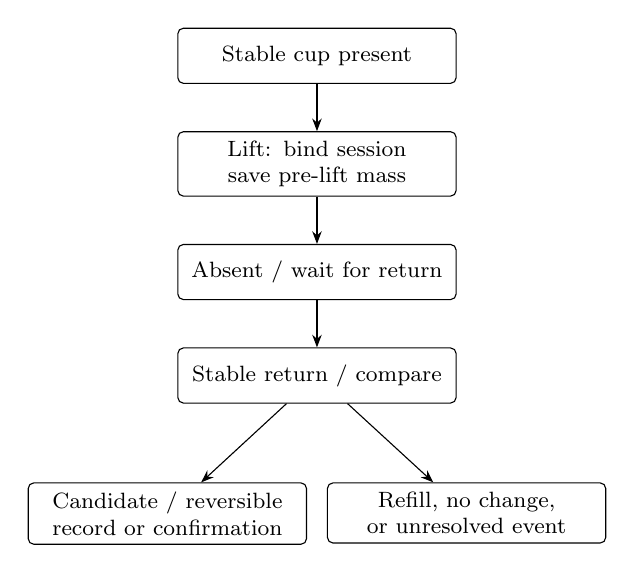
\begin{tikzpicture}[font=\footnotesize,box/.style={draw,align=center,rounded corners=2pt,text width=33mm,minimum height=7mm},arr/.style={-{Stealth[length=1.6mm]}}]
\node[box] (a) {Stable cup present};
\node[box,below=6mm of a] (b) {Lift: bind session\\save pre-lift mass};
\node[box,below=6mm of b] (c) {Absent / wait for return};
\node[box,below=6mm of c] (d) {Stable return / compare};
\node[box,below=10mm of d,xshift=-19mm] (e) {Candidate / reversible\\record or confirmation};
\node[box,below=10mm of d,xshift=19mm] (f) {Refill, no change,\\or unresolved event};
\draw[arr] (a)--(b);\draw[arr](b)--(c);\draw[arr](c)--(d);
\draw[arr](d)--(e);\draw[arr](d)--(f);
\end{tikzpicture}
\caption{\DIFaddFL{Proposed hydration workflow. The comparison creates an interpretable event; it cannot distinguish drinking from every other source of liquid loss.}}\label{fig:fsm}
\end{figure}


\DIFadd{For uncertainty estimates $u_b,u_a$ of the stable pre/post masses,
}\begin{equation}\DIFadd{u_{\Delta}^2=u_b^2+u_a^2-2\operatorname{Cov}(\bar m_b,\bar m_a).
\label{eq:uncertainty}}\end{equation}
\DIFadd{The root-sum-square shortcut is justified only if that covariance is negligible. Drift can correlate the observations; Eq.~\eqref{eq:uncertainty} specifies propagation, not an estimated confidence bound. E1 must estimate uncertainty before thresholds or detection limits are interpreted.
}

\DIFadd{A }\DIFaddend normal candidate may create a reversible inferred record\DIFdelbegin \DIFdel{. User-confirmed, inferred, corrected, and rejected events retain different statuses. Confirming an event records }\DIFdelend \DIFaddbegin \DIFadd{; ambiguous candidates require an authenticated user response. A confirmation is }\DIFaddend a human report, not \DIFdelbegin \DIFdel{independent physiological proof of ingestion. }%DIFDELCMD < 

%DIFDELCMD < \begin{figure}[t]
%DIFDELCMD < \centering
%DIFDELCMD < \begin{tikzpicture}[font=\footnotesize,box/.style={draw,align=center,rounded corners=2pt,text width=33mm,minimum height=7mm},arr/.style={-{Stealth[length=1.6mm]}}]
%DIFDELCMD < \node[box] (a) {Stable cup present};
%DIFDELCMD < \node[box,below=6mm of a] (b) {Lift: bind session\\save pre-lift mass};
%DIFDELCMD < \node[box,below=6mm of b] (c) {Absent / wait for return};
%DIFDELCMD < \node[box,below=6mm of c] (d) {Stable return / compare};
%DIFDELCMD < \node[box,below=10mm of d,xshift=-19mm] (e) {Candidate / reversible\\record or confirmation};
%DIFDELCMD < \node[box,below=10mm of d,xshift=19mm] (f) {Refill, no change,\\or unresolved event};
%DIFDELCMD < \draw[arr] (a)--(b);\draw[arr](b)--(c);\draw[arr](c)--(d);
%DIFDELCMD < \draw[arr](d)--(e);\draw[arr](d)--(f);
%DIFDELCMD < \end{tikzpicture}
%DIFDELCMD < %%%
%DIFDELCMD < \caption{%
{%DIFAUXCMD
\DIFdelFL{Proposed hydration workflow. The comparison creates an interpretable event; it cannot distinguish drinking from every other source of liquid loss.}}%DIFAUXCMD
%DIFDELCMD < \label{fig:fsm}
%DIFDELCMD < \end{figure}
%DIFDELCMD < 

%DIFDELCMD < %%%
\DIFdel{Each final record retains links to its pre/post observations, calibration version, candidate, and correction history. }\DIFdelend \DIFaddbegin \DIFadd{physiological ground truth. Preserve observation, candidate, disposition and correction links. Rejection or correction appends a revision rather than overwriting the original event. }\DIFaddend A spill can \DIFdelbegin \DIFdel{be observationally indistinguishable from a drink; the interface must permit undo and the evaluation must include such confounders. The correction does not erase the original estimate. Offline events retain identifiers on replay, and a repeated identifier must not create a second record}\DIFdelend \DIFaddbegin \DIFadd{still imitate a drink, so inferred totals must remain identifiable}\DIFaddend .

\subsection{Food \DIFdelbegin \DIFdel{Mass }\DIFdelend \DIFaddbegin \DIFadd{Quantities }\DIFaddend and \DIFdelbegin \DIFdel{Nutrient Semantics}\DIFdelend \DIFaddbegin \DIFadd{Current-Revision Totals}\DIFaddend }
For an identified single food \DIFdelbegin \DIFdel{, the user tares the container, places the food, and confirms its identity and net mass. For nutrient $j$,
}\begin{displaymath}\DIFdel{m_{\rm net}=m_{\rm gross}-m_{\rm tare},\qquad
\hat n_j=\frac{m_{\rm net}}{100\ {\rm g}}c_j,%DIFDELCMD < \label{eq:nutrition}%%%
}\end{displaymath}%DIFAUXCMD
\DIFdelend \DIFaddbegin \DIFadd{with known preparation state,
}\begin{equation}\DIFadd{\begin{aligned}
m_{\rm net}&=m_{\rm gross}-m_{\rm tare},\\
\hat n_j&=\frac{m_{\rm net}}{100\ {\rm g}}c_j,
\end{aligned}\label{eq:nutrition}}\end{equation}\DIFaddend 
where $c_j$ \DIFdelbegin \DIFdel{is the nutrient quantity }\DIFdelend \DIFaddbegin \DIFadd{carries nutrient $j$'s unit }\DIFaddend per 100 g\DIFdelbegin \DIFdel{for the selected food and preparation state. The backend preserves units, food identifier, source, and source version. FoodData Central is one documented source~\cite{usda}; a Taiwan food-composition source may be selected and verified during implementation. Missing composition is not a zeronutrient value. For mixed }\DIFdelend \DIFaddbegin \DIFadd{. Negative net mass, unstable input or an unknown tare is invalid and requires re-taring. An explicitly observed empty tared container can represent zero; unknown mass cannot. Retain food ID, preparation state, source release, quantity basis and units. Missing composition remains null, not zero. Mixed }\DIFaddend meals without component weights \DIFdelbegin \DIFdel{, reference portions are labeled estimates and are not passed through }\DIFdelend \DIFaddbegin \DIFadd{use visibly labeled reference portions rather than applying }\DIFaddend Eq.~\eqref{eq:nutrition} \DIFdelbegin \DIFdel{using unknown }\DIFdelend \DIFaddbegin \DIFadd{to }\DIFaddend container gross mass\DIFaddbegin \DIFadd{~\cite{usda}}\DIFaddend .

\DIFdelbegin \subsection{\DIFdel{Multi-User Session Consistency}}
%DIFAUXCMD
\addtocounter{subsection}{-1}%DIFAUXCMD
\DIFdel{Let a shared }\DIFdelend \DIFaddbegin \DIFadd{Let $\mathcal R(q)$ contain only the current, non-rejected revision of each logical intake record at snapshot $q$. Inferred and confirmed hydration are reported separately:
}\begin{equation}\DIFadd{H_s(I,q)=\sum_{\substack{r\in\mathcal R(q),\ t_r\in I\\\operatorname{status}(r)=s}} V_r,
\quad s\in\{\mathrm{inferred},\mathrm{confirmed}\}.\label{eq:totals}}\end{equation}
\DIFadd{Corrections supersede prior revisions atomically; a record contributes to at most one status partition. Nutrients sum only known compatible units over the same current revisions and return a missing-component count. A displayed total must identify partial coverage; it cannot imply complete dietary intake. Use unrounded backend quantities for sums and round only at presentation.
}

\subsection{\DIFadd{Coordinated Multi-User Session Switching}}
\DIFadd{A shared monotonic }\DIFaddend session version $v$ \DIFdelbegin \DIFdel{bind both scalesto an active user. An event stores $v_e=v(t_{\rm start})$. Its owner is resolved from the corresponding trusted session record, even if the active session changes before the cup returns. FastAPI must authenticate the device and validate that version rather than accept an arbitrary user field.
A transaction updates the active session and its monotonically increasing version }\DIFdelend \DIFaddbegin \DIFadd{covers both scales}\DIFaddend . \DIFdelbegin \DIFdel{Events whose session context cannot be verified are held for resolution, not reassigned to the current user. }\DIFdelend \DIFaddbegin \DIFadd{Each event binds $v_e=v(t_{\rm start})$ and its owner through a device-authenticated, server-issued grant; upload time never determines ownership. A backend transaction alone is insufficient when workers hold stale state. We therefore propose a switch barrier:
}\begin{enumerate}
\item \DIFadd{Pause new event starts on both workers. Each durably logs and acknowledges its in-flight event IDs, sequence watermark and old session version. Existing events may finish under that binding.
}\item \DIFadd{After both acknowledgements, FastAPI commits the new version using compare-and-swap. Historical in-flight bindings are retained; no version number is reused.
}\item \DIFadd{Install the new grant on both workers. Activate new starts only after both acknowledge installation; each worker must observe the activation before resuming.
}\end{enumerate}
\DIFadd{A lost pause/install acknowledgement or disconnected worker prevents activation; physical actions during the hold are marked unresolved. Failed attempts remain logged and any committed-but-inactive version is never silently rolled back or reused. Historical completions are accepted only for the registered event IDs and authenticated sequence context. Duplicate IDs are idempotent; conflicting payloads are rejected. A restarted worker must resynchronize grants before new starts, while recoverable durable in-flight events retain their original owner. Unrecognized old starts, expired grants and unverifiable replay are quarantined. Grant freshness limits and sequence persistence belong in the pre-test manifest. This trades availability for attributable records and requires future implementation tests.
}\DIFaddend 

\subsection{\DIFaddbegin \DIFadd{Consistent, Authorized }\DIFaddend Agent Retrieval\DIFdelbegin \DIFdel{and Numeric Grounding}\DIFdelend }
\DIFdelbegin \DIFdel{Figure~\ref{fig:tools} specifies the retrieval path. Tool arguments are schema-checked, date ranges are bounded , and query results are scoped to the authenticated requestor. The backend computes hydration totals and nutritional sums; the model explains those values with source identifiers.
A tool result includes its query interval, timezone, }\DIFdelend \DIFaddbegin \DIFadd{The retrieval flow in Fig.~\ref{fig:tools} uses six allowlisted read-only query functions (daily hydration, hydration history, food history, nutrition summary, goal progress and record sources). FastAPI derives the subject from authenticated user/service context; model-supplied identity is ignored for authorization. Tool requests validate schema, bounded date range and units before database access. Food descriptions and retrieved text are untrusted data and cannot issue tool instructions or expand the allowlist.
}

\DIFadd{A local day is $[d\ 00{:}00,(d+1)\ 00{:}00)$ in the declared IANA timezone, with each boundary converted to UTC. It is not assumed to be exactly 24 hours. Multi-day queries use the same half-open rule. A read-consistent database transaction supplies both totals and their source revisions at one snapshot $q$; concurrent correction must not mix old sources with new totals.
}

\DIFadd{Every result includes status, authorized subject binding, interval/timezone, snapshot identifier, }\DIFaddend units, completeness \DIFdelbegin \DIFdel{indicator, and provenance. An empty history produces a missing-data statement, while an observed zeroremains a numeric zero. No tool permits the model to modify an intake record or prescribe a medical treatment. Corrections remain explicit }\DIFdelend \DIFaddbegin \DIFadd{and missing counts, source record/revision IDs, quantity-basis and food/calibration versions where applicable, and tool/schema version. Daily response envelopes distinguish complete observed zero, no observations, partial coverage, denied access and upstream failure. Denied responses expose no other user's record existence or IDs. The model may summarize only returned facts; numeric and provenance consistency are checked separately in E5. Corrections are }\DIFaddend authenticated interface actions\DIFaddbegin \DIFadd{, never agent writes}\DIFaddend .

\begin{figure}[t]
\centering
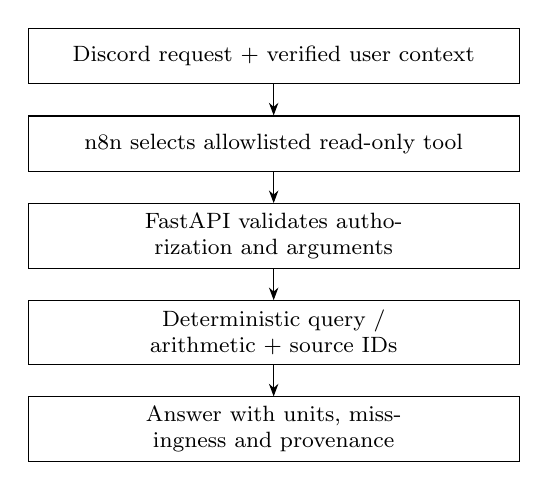
\begin{tikzpicture}[font=\footnotesize,box/.style={draw,align=center,text width=60mm,minimum height=7mm},arr/.style={-{Stealth[length=1.6mm]}}]
\node[box] (a) {Discord request + verified user context};
\node[box,below=4mm of a] (b) {n8n selects allowlisted read-only tool};
\node[box,below=4mm of b] (c) {FastAPI validates authorization and arguments};
\node[box,below=4mm of c] (d) {Deterministic query / arithmetic + source IDs};
\node[box,below=4mm of d] (e) {Answer with units, missingness and provenance};
\draw[arr](a)--(b);\draw[arr](b)--(c);\draw[arr](c)--(d);\draw[arr](d)--(e);
\end{tikzpicture}
\caption{Agent-tool workflow. A model-selected tool does not confer authorization; server checks precede data access.}\label{fig:tools}
\end{figure}


\section{Experimental Evaluation Plan}\label{sec:evaluation}
All experiments in this section are prospective. No measurement table, usability improvement, or agent success rate has been obtained for \sys{}. Table~\ref{tab:eval} separates the intended evidence from the research questions. Protocol decisions and actual calibration parameters must be recorded before collecting test data.

\begin{table}[t]
\caption{Prospective evaluation matrix; every result is pending.}\label{tab:eval}
\centering\footnotesize\setlength{\tabcolsep}{4pt}
\DIFdelbeginFL %DIFDELCMD < \begin{tabular}{@{}p{.08\columnwidth}p{.39\columnwidth}p{.44\columnwidth}@{}}%%%
\DIFdelendFL \DIFaddbeginFL \begin{tabular}{@{}P{.08\columnwidth}P{.39\columnwidth}P{.44\columnwidth}@{}}\DIFaddendFL \toprule
ID & Reference / comparison & Main measures\\\midrule
E1 & Known masses; independent reference balance & MAE, RMSE, maximum error, drift\\
E2 & Labeled physical actions; delta vs FSM vs confirmation & Precision, recall, F1, prompts\\
E3 & Scripted three-user, two-scale switches & Wrong attribution, success, latency\\
E4 & Matched tasks: manual vs semi-automatic & Time, actions, omissions, completion\\
E5 & Frozen tool fixtures and expected answers & Tool choice, values, sources, access safety\\\bottomrule
\end{tabular}
\end{table}

\subsection{E1: Weight Accuracy and Stability}
For each scale, reference loads spanning its documented operating range are placed repeatedly in randomized order. Record cold-start behavior, zero drift, settling time, and repeatability. Calibration and evaluation placements are kept separate. With errors $e_i=\hat m_i-m_i^*$ against an independent reference mass,
\begin{equation}\operatorname{MAE}=\frac{1}{N}\sum_{i=1}^N|e_i|,\quad
\operatorname{RMSE}=\sqrt{\frac{1}{N}\sum_{i=1}^Ne_i^2}.\label{eq:errors}\end{equation}
\DIFdelbegin \DIFdel{Report }\DIFdelend \DIFaddbegin \DIFadd{Propose five load levels $\{0,.2,.4,.6,.8\}M$ within documented capacity, five randomized placements per level in each of two sessions per scale: 50 test placements per scale. Calibration uses three separate placements at each of three reference levels (zero, $.4M$, $.8M$) and is fixed before that session's test block. Matching load values are allowed, but test placements are never used to fit coefficients. Record the exact physical masses, reference uncertainty, mounting and session conditions before collection. These are proposed counts, not completed trials. Report session/scale summaries and }\DIFaddend maximum absolute error as well. Reference-balance resolution and calibration uncertainty bound what can be inferred about the sensor. Test both assemblies rather than pooling them into an apparent increase in sample size.

\subsection{E2: Event Detection and Confirmation}
A labeled protocol includes drinking, lift-and-return without intake, refill, discard, spill, vessel change, and accidental contact. Ground truth combines a scripted action label, observer timing, and independently weighed transferred liquid. Ground-truth drink labels must not be produced by the same confirmation interface being evaluated. Compare (A) simple stable weight difference, (B) temporal FSM, and (C) FSM with human confirmation on the same observation traces. Retain all exclusions and timeouts.

\DIFaddbegin \DIFadd{Propose ten trials for each of the seven action classes, spread over two acquisition blocks, giving 70 action opportunities. Pilot/calibration traces are excluded. Freeze matching tolerance $\delta_t$ before test scoring using observer timing resolution and a justified timing allowance. Match predicted events to ground-truth ingestion events within $\delta_t$ of the labeled return using maximum-cardinality one-to-one matching; minimize total absolute time difference to break ties, then use event IDs. A matched event is TP, every unmatched recorded-ingestion prediction is FP (including duplicate detections), and every unmatched ground-truth drink is FN. Refills and spills are negative action opportunities; their false drink records count as FP. Unresolved/time-out drinks remain FN for final-record scoring, and unresolved coverage is reported separately. Also report specificity over labeled negative opportunities.
}

\DIFadd{Evaluate raw candidates and final records separately; ordinary inferred records count as final predictions unless rejected. Confirmation uses actual logged user responses, not oracle labels injected into the algorithm. A replay without such responses evaluates only the sensor stages. All methods see identical traces and fixed scoring rules. }\DIFaddend For matched events, report
\begin{equation}P=\frac{TP}{TP+FP},\quad R=\frac{TP}{TP+FN},\quad
F_1=\frac{2PR}{P+R}.\label{eq:detection}\end{equation}
Zero-denominator quantities are reported as undefined, not silently perfect. Report raw candidate performance separately from final recorded-intake performance. Count prompts, user corrections, and unresolved events. A high precision obtained by asking about every event must remain visible as interaction burden.

\subsection{E3: Shared-Device Attribution}
Three test users alternate control of both scales according to a scripted schedule. Include switches during an absent-cup interval, food weighing, and queued offline events. An external schedule establishes the intended event owner. Report wrong-owner records divided by attributable events, switch acknowledgement success, elapsed switch time, and unresolved events. \DIFaddbegin \DIFadd{Propose six scenarios (ordinary switch, mid-lift switch, duplicate replay, lost acknowledgement, disconnection and restart), each for three intended owners and both scales: 36 scripted attempts. The expected outcomes follow the switch barrier in Section~\ref{sec:method}, including holds rather than guessed owners. Alongside wrong-owner/resolved-record rate, report resolved coverage over all eligible events and wrong-owner/all-eligible rate. Report activated switches over all requested switches; failed attempts and missing acknowledgements remain in the denominator. }\DIFaddend Trace event IDs and session versions across retries. This is a consistency evaluation, not a measurement of identity recognition.

\subsection{E4: Recording Effort}
Use a within-person crossover pilot with the three intended users performing matched hydration and food tasks in manual and semi-automatic conditions. \DIFdelbegin \DIFdel{Counterbalance condition order as far as an odd-sized pilot permits and log the actual sequence}\DIFdelend \DIFaddbegin \DIFadd{Plan two sessions per participant, each with four matched tasks per condition (two hydration, two food). Use AB in one session and BA in the other, assigning the initial order before testing and rotating task variants: 16 planned tasks per person. Log actual order and deviations; training tasks are separate}\DIFaddend . Provide equivalent training and task quantities. Measure task time, explicit actions, omissions relative to the observer log, and completed tasks. Include confirmation and correction time, rather than counting only automatic records. \DIFdelbegin \DIFdel{Report paired }\DIFdelend \DIFaddbegin \DIFadd{Set a proposed 10-minute task deadline before collection. Retain timed-out tasks as incomplete with time reported as censored at the deadline; do not turn those into fast successful trials. Report each person's completion/omission proportions and median paired time differences for completed matched tasks, alongside counts of excluded incomplete pairs. Do not impute completion times or pool repeated tasks as independent people. Report paired }\DIFaddend participant-level summaries; this small convenience sample supports feasibility observations, not population-level effectiveness claims.

\subsection{E5: Agent Reliability and Authorization}
\DIFdelbegin \DIFdel{Prepare at least }\DIFdelend \DIFaddbegin \DIFadd{Propose }\DIFaddend 30 \DIFdelbegin \DIFdel{fixed casesacross daily and }\DIFdelend \DIFaddbegin \DIFadd{frozen cases: five each for daily hydration, }\DIFaddend multi-day hydration, nutrition, compound queries, missing/conflicting data, and authorization/\DIFdelbegin \DIFdel{safety requests. Each case specifies the authenticated subject, fixture records, expected tool behavior, permitted data, numeric answers and provenance. Run each case repeatedly with the modelidentifier, }\DIFdelend \DIFaddbegin \DIFadd{adversarial requests. Run each case three times from a reset fixture and conversation, for 90 planned runs. Freeze model/provider identifier, sampling settings, }\DIFaddend prompt, tool schema, \DIFdelbegin \DIFdel{sampling settings, and workflow version recorded. Following the motivation of repeated agentevaluation~\cite{yao2024tau}, report both per-run correctness and consistency across repeats. Unauthorized disclosure is a failure even when a numeric answer is
otherwise correct }\DIFdelend \DIFaddbegin \DIFadd{workflow version and fixture hash. Include day-boundary queries, a corrected source revision, malicious source text, forged identities, unavailable tools and upstream failures. These are test stimuli, not observations of a running agent}\DIFaddend .
\DIFaddbegin 

\DIFadd{A deterministic oracle computes quantities from the fixture's authorized current revisions and accepted unit conversions. Freeze acceptable tool-call sequences (including equivalent permitted alternatives), rounding rules and expected statuses before runs. Score tool correctness $T_{ik}$, numeric/status correctness $N_{ik}$, source/version correctness $P_{ik}$ and authorization/safety $A_{ik}$ as binary components for case $i$, repeat $k$. Numeric tolerance is half of the declared last displayed unit after canonical conversion; no-data cases require the expected nonnumeric status, not a fabricated zero. An unauthorized call attempt fails $A_{ik}$ even if the backend denies it; backend non-disclosure is reported as a separate defense check. Strict run success is
}\begin{equation}\DIFadd{S_{ik}=T_{ik}N_{ik}P_{ik}A_{ik},\quad
\bar S=\frac{1}{90}\sum_{i=1}^{30}\sum_{k=1}^{3}S_{ik}.\label{eq:agent}}\end{equation}
\DIFadd{Report component rates and family-level counts as well as empirical all-three-repeat case reliability,
}\begin{equation}\DIFadd{C_3=\frac{1}{30}\sum_{i=1}^{30}\prod_{k=1}^{3}S_{ik}.\label{eq:repeat}}\end{equation}
\DIFadd{This read-only metric is inspired by repeated evaluation~\cite{yao2024tau}, not a reproduction of its state-changing benchmark. Grade final answers and returned sources against the oracle, not by another unconstrained LLM. Have a second evaluator check semantic/adversarial judgments and record disagreements. Refusals and missing-data statements must match the case's expected policy. A correct number cannot compensate for wrong provenance or a privacy failure. }\DIFaddend No clinical safety \DIFdelbegin \DIFdel{claim follows from a small scripted benchmark}\DIFdelend \DIFaddbegin \DIFadd{guarantee follows from this small scripted suite}\DIFaddend .

\subsection{Reproducibility and Data Handling}
Before execution, freeze sensor parameters, software versions, stimulus schedules, case definitions and analysis rules. \DIFaddbegin \DIFadd{Keep acquisition-block and case identifiers for clustered descriptive summaries; do not treat temporally adjacent sensor windows or repeated agent runs as independent participants. Planned counts are feasibility choices, not a power calculation. }\DIFaddend Save de-identified traces with record and correction relationships. Participant consent and applicable institutional review must precede real personal-data collection. Raw health records and identifiable screenshots do not belong in the public release. Disclose missing trials, device failures, exclusions and changes to the protocol.

\section{Discussion and Limitations}\label{sec:discussion}
The architecture makes three separations explicit: mass change from ingestion, physical device ownership from query identity, and language generation from backend facts. These separations expose errors that could otherwise disappear inside a daily total. However, preserving an error's provenance does not prevent the error. Confirmation can be ignored, a reference portion can be inappropriate, and a correct tool result can be misrepresented in the final response.

The fixed setting limits coverage: intake outside the scales requires manual entry. Cup mass cancellation assumes a consistent vessel, and changes in mounting, vibration or temperature may degrade calibration. Multi-user switching introduces a coordination step that must be included in the usability comparison. A three-person pilot cannot establish general adoption or clinical benefit. Nutrition estimates are constrained by food identification, preparation state, source coverage and portion assumptions.

Tool grounding reduces reliance on model arithmetic but leaves tool selection, argument interpretation, timezone handling and explanation quality as separate risks. Prompt injection or malicious food descriptions must not widen access. Security claims require adversarial tests of actual endpoints, credentials and database policies; architecture diagrams alone are insufficient evidence. Goals should be user-configured and not presented as medical prescriptions.

This manuscript reports a design and prospective methodology. The authorized project documentation describes planned integration; no running prototype, deployed interface or formal E1--E5 result is independently verified here. Image-based food estimation, external health-record imports, wellness scores, LINE support and dashboards remain outside the stated MVP evidence. Those extensions should not be used to imply current completeness.

\DIFaddbegin \DIFadd{The switch barrier deliberately sacrifices availability during an unacknowledged transition; E3 reports this coverage cost alongside wrong attribution. Three users and two acquisition sessions per scale offer only a feasibility sample. Neither repeated agent calls nor repeated task placements increase the number of independent people. The additional lifecycle, snapshot and scoring rules are proposed contracts: their presence in this manuscript is not evidence that concurrent software, hardware behavior or access policies have passed tests.
}

\DIFaddend \section{Conclusion}\label{sec:conclusion}
\sys{} proposes an IoT and tool-grounded agent architecture for hydration and dietary recording in fixed workplaces. Two scales support candidate-event sensing and food weighing, while server-enforced sessions, deterministic analytics and provenance-aware summaries address attribution and interpretation. The E1--E5 plan separates measurement, detection, interaction and agent reliability so that future evaluation can test the claimed benefits without treating an accurate mass difference as proof of ingestion. Implementation verification and measured results are the next research steps; no effectiveness or clinical outcome is claimed.

\balance
\bibliographystyle{IEEEtran}
% Generated by IEEEtran.bst, version: 1.14 (2015/08/26)
\begin{thebibliography}{1}
\providecommand{\url}[1]{#1}
\urlstyle{same}
\providecommand{\newblock}{\relax}
\providecommand{\bibinfo}[2]{#2}
\providecommand{\BIBentrySTDinterwordspacing}{\spaceskip=0pt\relax}
\providecommand{\BIBentryALTinterwordstretchfactor}{4}
\providecommand{\BIBentryALTinterwordspacing}{\spaceskip=\fontdimen2\font plus
\BIBentryALTinterwordstretchfactor\fontdimen3\font minus \fontdimen4\font\relax}
\providecommand{\BIBforeignlanguage}[2]{{%
\expandafter\ifx\csname l@#1\endcsname\relax
\typeout{** WARNING: IEEEtran.bst: No hyphenation pattern has been}%
\typeout{** loaded for the language `#1'. Using the pattern for}%
\typeout{** the default language instead.}%
\else
\language=\csname l@#1\endcsname
\fi
#2}}
\providecommand{\BIBdecl}{\relax}
\BIBdecl

\bibitem{burke2011}
\DIFaddbegin \BIBentryALTinterwordspacing
\DIFaddend L.~E. Burke, J.~Wang, and M.~A. Sevick, ``Self-monitoring in weight loss: A systematic review of the literature,'' \emph{Journal of the American Dietetic Association}, vol. 111, no.~1, pp. 92--102, 2011. \DIFaddbegin [\DIFadd{Online}]\DIFadd{. Available: }\url{https://doi.org/10.1016/j.jada.2010.10.008}
\BIBentrySTDinterwordspacing
\DIFaddend 

\bibitem{cohen2022}
\DIFaddbegin \BIBentryALTinterwordspacing
\DIFaddend R.~Cohen, G.~Fernie, and A.~{Roshan Fekr}, ``Monitoring fluid intake by commercially available smart water bottles,'' \emph{Scientific Reports}, vol.~12, no.~1, p. 4402, 2022. \DIFaddbegin [\DIFadd{Online}]\DIFadd{. Available: }\url{https://doi.org/10.1038/s41598-022-08335-5}
\BIBentrySTDinterwordspacing
\DIFaddend 

\bibitem{yao2023react}
\BIBentryALTinterwordspacing
S.~Yao, J.~Zhao, D.~Yu, N.~Du, I.~Shafran, K.~Narasimhan, and Y.~Cao, ``{ReAct}: Synergizing reasoning and acting in language models,'' in \emph{International Conference on Learning Representations}, 2023, camera-ready version v3. [Online]. Available: \url{https://arxiv.org/abs/2210.03629}
\BIBentrySTDinterwordspacing

\bibitem{schick2023}
T.~Schick, J.~Dwivedi-Yu, R.~Dess{\`i}, R.~Raileanu, M.~Lomeli, L.~Zettlemoyer, N.~Cancedda, and T.~Scialom, ``Toolformer: Language models can teach themselves to use tools,'' arXiv:2302.04761, 2023.

\bibitem{chiu2009}
\DIFaddbegin \BIBentryALTinterwordspacing
\DIFaddend M.-C. Chiu, S.-P. Chang, Y.-C. Chang, H.-H. Chu, C.~C.-H. Chen, F.-H. Hsiao, and J.-C. Ko, ``Playful bottle: A mobile social persuasion system to motivate healthy water intake,'' in \emph{Proceedings of the 11th International Conference on Ubiquitous Computing}, 2009, pp. 185--194. \DIFaddbegin [\DIFadd{Online}]\DIFadd{. Available: }\url{https://doi.org/10.1145/1620545.1620574}
\BIBentrySTDinterwordspacing
\DIFaddend 

\bibitem{usda}
\BIBentryALTinterwordspacing
{USDA Agricultural Research Service}, ``{FoodData Central}: Data type documentation,'' Online documentation, accessed: Nov. 25, 2026. [Online]. Available: \url{https://fdc.nal.usda.gov/data-documentation/}
\BIBentrySTDinterwordspacing

\bibitem{yao2024tau}
S.~Yao, N.~Shinn, P.~Razavi, and K.~Narasimhan, ``{\(\tau\)}-bench: A benchmark for tool-agent-user interaction in real-world domains,'' arXiv:2406.12045, 2024.

\bibitem{prov}
\BIBentryALTinterwordspacing
L.~Moreau and P.~Missier, ``{PROV-DM}: The {PROV} data model,'' World Wide Web Consortium, W3C Recommendation, Apr. 2013, editors. [Online]. Available: \url{https://www.w3.org/TR/prov-dm/}
\BIBentrySTDinterwordspacing

\end{thebibliography}

\end{document}
